\subsection{Đánh giá mô hình dịch Việt - Lào}

Khác với mô-đun ghép câu tiếng Việt, mô-đun dịch Việt - Lào là một bài toán dịch máy đa
ngôn ngữ. Vì vậy, việc đánh giá cần bám theo các metric chuẩn của machine translation,
đồng thời phải đi kèm các ví dụ định tính để tránh hiểu sai các con số.

\subsubsection{Các metric nên sử dụng}

Ba metric tự động quan trọng nhất cho cặp Việt - Lào trong đồ án này là:
\begin{itemize}
    \item \textbf{BLEU}: metric cổ điển của Papineni và cộng sự, dựa trên độ trùng
    \textit{modified n-gram precision}. BLEU phù hợp để so sánh tương đối giữa các lần
    huấn luyện hoặc giữa các cấu hình mô hình.
    \item \textbf{chrF}: metric của Popovi\'{c}, dựa trên F-score của \textit{character
    n-gram precision/recall}. Với các ngôn ngữ có hệ chữ viết riêng hoặc dễ phát sinh khác
    biệt hình thức bề mặt, chrF thường phản ánh tốt hơn BLEU ở mức ký tự.
    \item \textbf{TER}: metric của Snover và cộng sự, đo số phép chỉnh sửa tối thiểu cần để
    biến câu dự đoán thành câu tham chiếu. Khác với BLEU và chrF, TER là metric
    \textit{càng thấp càng tốt}.
\end{itemize}

Ngoài ba metric trên, đối với một hệ thống hỗ trợ giao tiếp, nên bổ sung:
\begin{itemize}
    \item \textbf{đánh giá thủ công về adequacy} (mức bảo toàn ý nghĩa);
    \item \textbf{đánh giá thủ công về fluency} (độ tự nhiên của câu tiếng Lào);
    \item \textbf{kiểm tra lỗi tên riêng, số, địa danh và câu mệnh lệnh}, vì đây là các trường
    hợp rất dễ ảnh hưởng đến khả năng dùng trong thực tế.
\end{itemize}

\begin{table}[H]
\centering
\caption{Ý nghĩa của các metric đánh giá mô-đun dịch Việt - Lào}
\begin{tabularx}{\textwidth}{|p{2.5cm}|X|X|}
\hline
\textbf{Metric} & \textbf{Ý nghĩa} & \textbf{Cách diễn giải} \\
\hline
BLEU & Độ trùng n-gram giữa câu dịch dự đoán và câu tham chiếu. & Càng cao càng tốt; phù hợp để so sánh các cấu hình mô hình. \\
\hline
chrF & Độ giống nhau ở cấp ký tự và recall/precision. & Càng cao càng tốt; hữu ích với ngôn ngữ ít tài nguyên hoặc khác hệ chữ. \\
\hline
TER & Số phép sửa tối thiểu để đưa dự đoán về câu chuẩn. & Càng thấp càng tốt; càng ít phải hậu biên tập. \\
\hline
Adequacy & Mức độ bảo toàn ý nghĩa so với câu nguồn. & Nên chấm thủ công theo thang 1--5. \\
\hline
Fluency & Độ tự nhiên của câu đích đối với người đọc bản ngữ. & Nên chấm thủ công theo thang 1--5. \\
\hline
\end{tabularx}
\end{table}

\subsubsection{Giao thức đánh giá nên áp dụng cho project}

Với dữ liệu hiện có trong repository, đánh giá chuẩn cho mô-đun dịch nên được thực hiện
trên đúng ba tập dữ liệu đã chia sẵn:
\begin{itemize}
    \item train: 90.000 cặp câu;
    \item validation: 5.000 cặp câu;
    \item test: 5.000 cặp câu.
\end{itemize}

Trên tập test, quy trình nên gồm các bước:
\begin{enumerate}
    \item sinh câu tiếng Lào cho toàn bộ 5.000 câu nguồn tiếng Việt bằng chính cấu hình
    inference đang dùng trong \texttt{translate.py};
    \item so sánh câu dự đoán với câu tham chiếu tiếng Lào bằng BLEU, chrF và TER;
    \item chọn khoảng 30 đến 50 câu đại diện ở các nhóm ngắn, dài, có tên riêng và có từ
    chuyên biệt để đánh giá định tính;
    \item đối chiếu thêm lỗi lan truyền từ mô-đun ghép câu nếu đánh giá end-to-end.
\end{enumerate}

\begin{table}[H]
\centering
\caption{Kết quả đánh giá định lượng mô-đun dịch Việt -- Lào trích từ \texttt{vilo.pdf}}
\label{tab:translation-eval-status}
\begin{tabularx}{\textwidth}{|X|c|X|}
\hline
\textbf{Chỉ số} & \textbf{Giá trị} & \textbf{Ý nghĩa} \\
\hline
Train loss & 4,67 & Mức độ lỗi trong quá trình huấn luyện. \\
\hline
Validation loss & 1,06 & Mức độ lỗi trên tập validation. \\
\hline
BLEU trên tập kiểm thử & 23,57 & Mức độ giống giữa bản dịch của mô hình và bản dịch chuẩn. \\
\hline
\end{tabularx}
\end{table}

\begin{figure}[H]
\centering
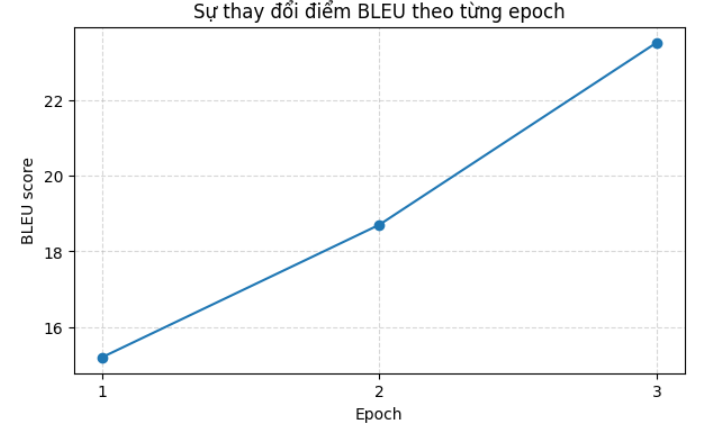
\includegraphics[width=0.78\textwidth]{figures/Anh/BLEU.png}
\caption{Sự thay đổi BLEU của mô-đun dịch Việt -- Lào theo từng epoch}
\label{fig:translation-bleu-epochs}
\end{figure}

\subsubsection{Nhận xét dựa trên trạng thái repository hiện tại}

Tại thời điểm viết báo cáo, snapshot mã nguồn hiện có:
\begin{itemize}
    \item bộ dữ liệu train/validation/test đã chia sẵn;
    \item adapter LoRA đã huấn luyện;
    \item script suy luận cho từng câu đầu vào.
    \item tài liệu \texttt{vilo.pdf} ghi nhận Train loss = 4,67, Validation loss = 1,06 và BLEU = 23,57.
\end{itemize}

Kết quả BLEU = 23,57 cho thấy mô hình đã học được khả năng dịch tương đối cho cặp Việt -- Lào, đặc biệt trong bối cảnh dữ liệu song ngữ ít tài nguyên hơn các cặp ngôn ngữ phổ biến. Tuy nhiên, mức BLEU này chưa phải chất lượng cao tuyệt đối; khi triển khai thực tế vẫn cần đánh giá thêm bằng ví dụ định tính và kiểm tra lỗi trên các câu dài, tên riêng, số và câu khẩu ngữ.

Trong workspace hiện tại chưa thấy số liệu chrF và TER tương ứng với cùng lần đánh giá. Vì vậy, cách trình bày trung thực nhất trong báo cáo là:
\begin{itemize}
    \item mô tả rõ mô hình đang dùng là \texttt{NLLB-200 Distilled 600M + LoRA};
    \item công bố các số liệu có nguồn trong \texttt{vilo.pdf}: Train loss, Validation loss và BLEU;
    \item giữ chrF và TER ở mức giao thức đề xuất, chưa công bố số nếu chưa tái lập được phép đo;
    \item tránh bịa thêm số liệu không có khả năng truy vết trong workspace.
\end{itemize}

Điểm này không phải là thiếu sót về học thuật, miễn là báo cáo ghi rõ trạng thái hiện tại và
không trình bày các con số không có khả năng truy vết.

\subsubsection{Đánh giá định tính nên nhấn mạnh điều gì}

Ngay cả khi đã có BLEU, chrF và TER, phần dịch Việt -- Lào vẫn cần thêm một bảng ví
dụ để người đọc thấy những kiểu lỗi quan trọng. Các nhóm ví dụ ưu tiên gồm:
\begin{itemize}
    \item câu nhu cầu cơ bản ngắn, ví dụ \textit{Tôi muốn uống nước};
    \item câu có tên riêng như bệnh viện, địa danh, tên người;
    \item câu dài hơn có mệnh đề phụ, ví dụ câu mô tả tình trạng sức khỏe hoặc yêu cầu trợ
    giúp;
    \item câu chứa số, thời gian hoặc thực thể viết hoa.
\end{itemize}

Quan sát nhanh trên dữ liệu song ngữ hiện có cho thấy các điểm rủi ro lớn nhất của mô-đun
dịch là:
\begin{itemize}
    \item tên riêng và từ phiên âm dễ bị sai hình thức;
    \item câu dài dễ lặp lại hoặc diễn đạt rườm rà;
    \item dữ liệu huấn luyện nhiều miền có thể làm mô hình không đồng đều chất lượng giữa
    các kiểu câu.
\end{itemize}

\subsubsection{Ý nghĩa của đánh giá đối với toàn hệ thống}

Mô-đun dịch là tầng cuối cùng trước khi thông tin đến tay người dùng đích. Vì vậy, nếu
mô-đun này dịch sai nghĩa, toàn bộ giá trị của pipeline trước đó có thể bị giảm mạnh. Đó là
lý do phần đánh giá dịch Việt - Lào cần được xem như một bước kiểm chứng độc lập và
đồng thời là một bước kiểm chứng cho chất lượng của cả hệ thống end-to-end.

